\section{Introduction}
Computer aided evolution(CAE) operates within the domain of evolutionary biology, in the sense that it attempts to replicate the darwinistic view, namely evolution by natural selection and survival of the fittest\cite{paper:ev3}.

Genetic algorithms provide a Darwinian framework for local search algorithms.
Dividing the sub problems of optimization into encoding, selection
n, and evaluation\cite{paper:ev3}.
\todo[inline]{expand (a little) on general bio evo, and how it transfers to
compsci}

Ultimately the goal with such evolution in our case is to develop candidates
which are not the most obvious design choices from a human perspective, but
score a higher grade compared to already known solutions.

\todo[inline]{dette kunne muligvis rykkes til previous work istedet}
An example of such results are space antennas developed by Gregory S. Hornby\cite{paper:ev4} using generative Computer-Automated Evolutionary Design[See figure \ref{fig:nasa_antenna}].
These antennas have rather controversal designs compared to the traditional archetype of an antenna.
\todo[inline]{Move example and figures out of introduction, they belong
elsewhere me thinks}

\begin{figure}[ht]
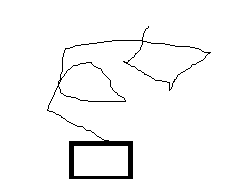
\includegraphics[scale=.7]{content/img/space_antenna}
\caption{Image of the NASA Antenna \cite{paper:ev4} }
\label{fig:nasa_antenna}
\end{figure}

Building from such previous experiences, that something which usually has a standardized morphology can get so fundamentally different results when applying CAE, leads us to wanting to apply such methodology to other domains.

The chosen domain is within furniture, namely the types which should be suited for seating.

One might wonder why this is relevant in our current time or in the future?

By being able to produce solutions which are outside of traditional design norms some of the problems in modern society can be dealt with, problems such as high resource consumption and strain on the environment when treating the resources.

Since there is a finite amount of raw materials and treatment of aforementioned  resources in the general case results in strain on the environment be it foraging for wood or producing plastics this project is deemed highly relevant.
\todo[inline]{I would scratch this, and justify the evo of furniture with the
claim that it is a classical design issue, and that it is complex enough to test
the bounderies (maybe too strong a claim) of evolution}

By tweaking the parameters to optimize for material or comfort, the candidate solutions might provide some very interesting and hopefully revolutionary designs.

Designs which ultimately might save the world.
\todo[inline]{No world saving and revolutionizing please, such claims only
antagonize the people who actually work in the field}
